% IA 642 Defensive Security
% Week 05 Bonus Lab: Seeing the Graph — STIX / TAXII Visualization
% Authors: Unais Ali (E02805019) and Hafiz Usama (E02574092)
% Submit as: Ali_Week05_Bonus_Lab_STIX_TAXII.pdf
\documentclass[11pt,letterpaper]{article}

\usepackage[margin=0.85in]{geometry}
\sloppy
\emergencystretch=3em
\usepackage{array}
\usepackage{booktabs}
\usepackage{tabularx}
\usepackage{enumitem}
\usepackage{parskip}
\usepackage{ragged2e}
\usepackage{titlesec}
\usepackage{graphicx}
\usepackage{float}
\usepackage{placeins}
\usepackage{microtype}
\usepackage{xcolor}
\usepackage{colortbl}
\usepackage{listings}
\usepackage{caption}
\usepackage{needspace}
\usepackage[colorlinks=true,linkcolor=blue,citecolor=blue,urlcolor=blue]{hyperref}
\usepackage{xurl}

\hypersetup{pdfauthor={Unais Ali; Hafiz Usama}, pdftitle={IA 642 Week 05 Bonus Lab STIX TAXII Visualization}}

\graphicspath{{captures/}{evidence/}{./}}

\definecolor{tblhead}{HTML}{1F4E79}
\definecolor{tblrow}{HTML}{F0F4F8}
\definecolor{codebg}{HTML}{F7FAFC}
\definecolor{okbox}{HTML}{E6F4EA}
\setlength{\parindent}{0pt}
\renewcommand{\arraystretch}{1.22}
\raggedbottom
\setlist[itemize]{leftmargin=1.2em,itemsep=0.22em,topsep=0.3em,parsep=0pt}
\setlist[enumerate]{leftmargin=1.3em,itemsep=0.28em,topsep=0.3em,parsep=0pt}
\newcolumntype{Y}{>{\RaggedRight\arraybackslash}X}

\titleformat{name=\section,numberless}{\large\bfseries\color{tblhead}\filright}{}{0em}{}
\titlespacing*{name=\section,numberless}{0pt}{0.85em}{0.3em}
\titleformat{name=\subsection,numberless}{\normalsize\bfseries\color{tblhead}\filright}{}{0em}{}
\titlespacing*{name=\subsection,numberless}{0pt}{0.55em}{0.2em}

\newcommand{\labpart}[1]{%
  \par\vspace{0.35em}%
  \Needspace{8\baselineskip}%
  \section*{#1}%
  \nopagebreak
}
\newcommand{\labstep}[1]{%
  \Needspace{6\baselineskip}%
  \subsection*{#1}%
  \nopagebreak
}

\lstset{
  basicstyle=\ttfamily\scriptsize,
  backgroundcolor=\color{codebg},
  frame=single,
  rulecolor=\color{tblhead},
  breaklines=true,
  breakatwhitespace=false,
  columns=fullflexible,
  keepspaces=true,
  showstringspaces=false,
  aboveskip=0.35em,
  belowskip=0.35em,
  xleftmargin=0.15em,
  framexleftmargin=0.2em
}

\newcommand{\evidencebox}[2]{%
  \par\vspace{0.25em}%
  \noindent\colorbox{okbox}{\parbox{\dimexpr\linewidth-2\fboxsep\relax}{%
    \textbf{Evidence \#{#1}.} #2}}%
  \par\vspace{0.25em}%
}

\begin{document}

\begin{center}
{\LARGE\bfseries IA 642 Defensive Security}\\[0.25em]
{\Large Week 05 Bonus / Extra Credit Lab}\\[0.2em]
{\large Seeing the Graph: Visualizing and Sharing Meridian's STIX Intelligence}\\[0.35em]
{\small Cyber Threat Intelligence Tooling --- STIX 2.1 $\cdot$ stix2viz $\cdot$ TAXII 2.1}\\[0.25em]
{\small Repository:
\href{https://github.com/unaisshazan/ia642-week05-lab51-cti/tree/master/Lab5_Bonus_Assignment}{github.com/unaisshazan/ia642-week05-lab51-cti/Lab5\_Bonus\_Assignment}}\\[0.25em]
\end{center}

\begin{tabularx}{\textwidth}{@{}l X l l@{}}
\toprule
\textbf{Group members} & Unais Ali & \textbf{EID} & E02805019 \\
 & Hafiz Usama &  & E02574092 \\
\textbf{Course} & IA 642 Defensive Security & \textbf{Week} & 05, Bonus Lab \\
\textbf{Tools} & stix2-validator, stix2viz, medallion, taxii2-client & \textbf{Date} & October 2026 \\
\bottomrule
\end{tabularx}

\vspace{0.55em}

\section*{Lab overview}

This bonus lab takes the closed Week~04 Kerberoasting / \texttt{svcupdate.bin} case and runs the full CTI tooling loop: author a STIX~2.1 bundle, validate it against the OASIS schema (not just \texttt{json.tool}), render it as a node-and-edge graph in OASIS \texttt{stix2viz}, serve it from a live TAXII~2.1 \texttt{medallion} collection, pull it back with \texttt{taxii2-client}, then extend the feed and re-verify end to end.

\begin{tabularx}{\textwidth}{@{}l Y@{}}
\toprule
\textbf{Host} & \textbf{Role} \\
\midrule
Analysis host (Python 3.11) & Authoring, validation, stix2viz HTTP server, medallion TAXII server, taxii2-client consumer \\
\bottomrule
\end{tabularx}

\labpart{1. Part A --- Assemble and validate the bundle}

\labstep{Step 1 --- Bundle contents}

The hand-authored bundle \texttt{meridian\_week4\_intel.json} contains six STIX~2.1 objects:

\begin{enumerate}
  \item Identity SDO --- Meridian Health Network SOC
  \item Malware SDO --- MeridianLoader (\texttt{is\_family=true}, type \texttt{downloader})
  \item Attack-Pattern SDO --- Kerberoasting with ATT\&CK \texttt{T1558.003}
  \item Indicator SDO --- pattern \texttt{[file:name = 'svcupdate.bin']}
  \item Relationship SRO --- \texttt{indicates} (indicator $\rightarrow$ malware)
  \item Relationship SRO --- \texttt{uses} (malware $\rightarrow$ attack-pattern)
\end{enumerate}

\texttt{python -m json.tool} reported well-formed JSON before schema validation.

\labstep{Step 2 --- OASIS stix2-validator}

Validator run used STIX~2.1 schemas from the OASIS \texttt{cti-stix2-json-schemas} repository (\texttt{stix2.1} branch). The pip wheel alone does not ship schemas; pointing \texttt{stix2\_validator --version 2.1 -s <schemas>} is required for a real schema check.

\evidencebox{1}{Full \texttt{stix2\_validator} output on the original six-object bundle:}

\begin{lstlisting}
================================================================================
[-] Results for: meridian_week4_intel.json
[+] STIX JSON: Valid
    [!] Warning: attack-pattern--3f1a2b4c-0003-4a7b-8c9d-000000000003:
        {302} External reference 'mitre-attack' has a URL but no hash.
\end{lstlisting}

\textbf{Interpretation.} The bundle is schema-valid with zero errors. The single residual SHOULD-warning~\{302\} is the expected mitre-attack external-reference hash advisory called out in the lab prompt; MITRE's own ATT\&CK references typically omit a hash as well, so it was left as-is. No other warnings remained.

\labpart{2. Part B --- Visualize the bundle as a graph}

\labstep{Step 3 --- OASIS stix2viz}

\texttt{cti-stix-visualization} was served locally with \texttt{python -m http.server 8080} and the original bundle was loaded in the browser at \texttt{http://127.0.0.1:8080/}.

\evidencebox{2}{Rendered graph (OASIS stix2viz) --- original six-object bundle:}

\begin{center}
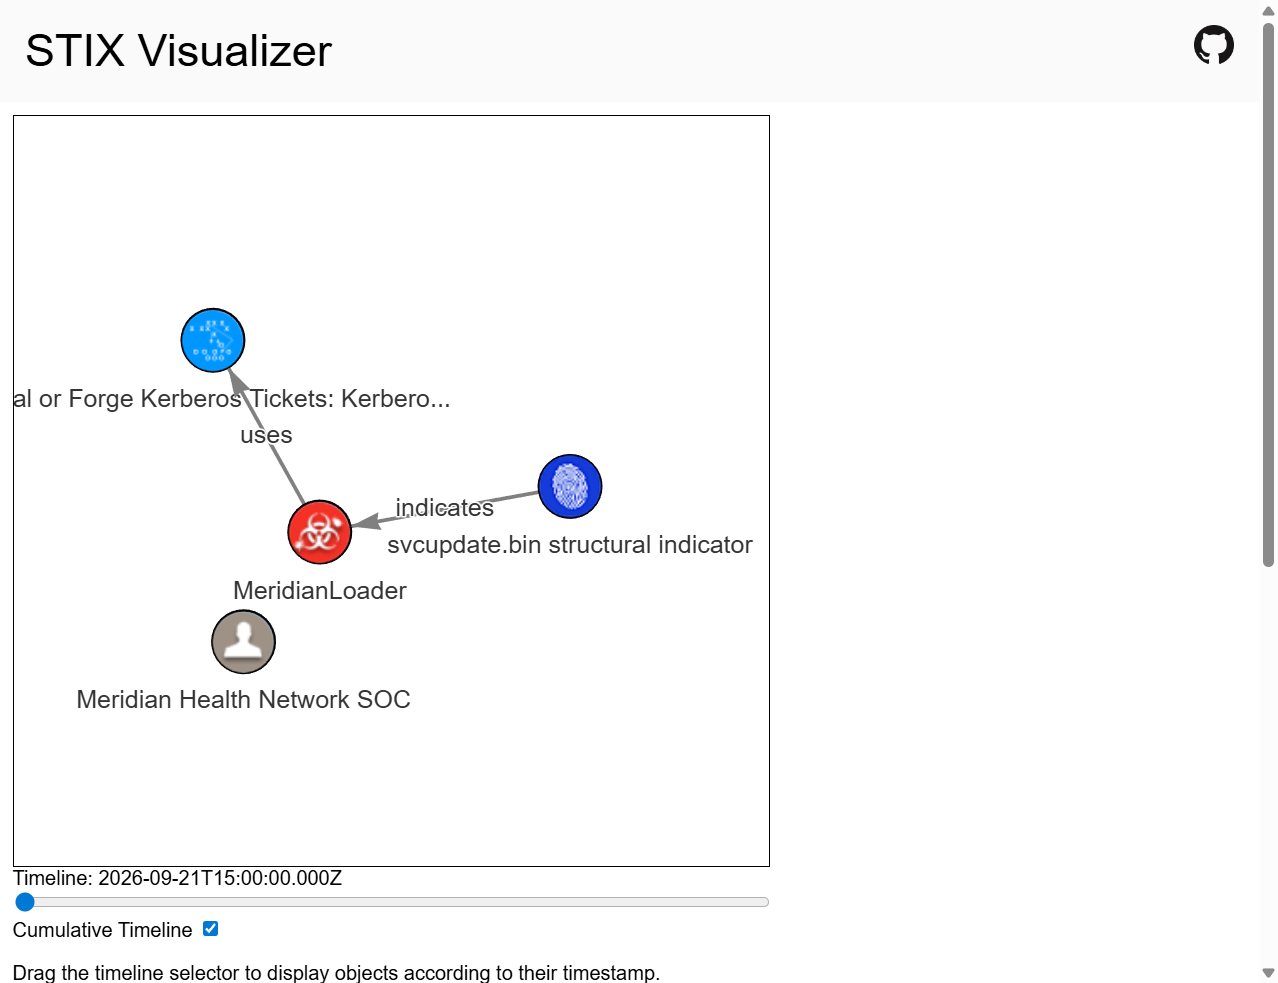
\includegraphics[width=0.92\textwidth,height=0.42\textheight,keepaspectratio]{stix2viz_original_graph.png}
\end{center}

\textbf{Graph reading.}
\begin{itemize}
  \item \textbf{Nodes (SDOs):} 4 --- Identity, Malware (\texttt{MeridianLoader}), Attack-Pattern (Kerberoasting), Indicator (\texttt{svcupdate.bin}).
  \item \textbf{Edges (SROs):} 2 --- \texttt{indicates} and \texttt{uses}.
  \item \textbf{Most-connected node:} Malware \texttt{MeridianLoader} (degree~2). The Identity node is present but unlinked (no \texttt{created\_by\_ref} / authorship edges in this minimal bundle).
\end{itemize}

\textbf{Malware node property panel contents:}
\begin{lstlisting}
type: malware
spec_version: 2.1
id: malware--3f1a2b4c-0002-4a7b-8c9d-000000000002
created / modified: 2026-09-21T15:00:00.000Z
name: MeridianLoader
is_family: true
malware_types: ["downloader"]
description: Loader recovered as svcupdate.bin from BILL-WS-14.
  Detected by YARA rule Meridian_SvcUpdate_Loader.
\end{lstlisting}

\labstep{Critical thinking \#1}

In this six-object bundle the \textbf{Malware} SDO (\texttt{MeridianLoader}) is the hub: both SROs touch it (\texttt{indicates} inbound from the Indicator; \texttt{uses} outbound to the Attack-Pattern). Relationship direction matters because STIX edges are typed and oriented. Reading \texttt{source\_ref $\rightarrow$ target\_ref} correctly distinguishes ``the indicator indicates the malware'' from the reverse claim, and ``the malware uses Kerberoasting'' from implying that the technique somehow contains the malware. Wrong direction would invert the analytic meaning even if the same two nodes were drawn next to each other.

\labpart{3. Part C --- Stand up a TAXII 2.1 server}

\labstep{Steps 4--6 --- medallion}

\texttt{medallion}~v3.0.0 was installed and configured with a memory backend whose \texttt{server\_data.json} wraps the six (later eight) STIX objects in one Collection. Discovery was confirmed with Basic auth and the mandatory TAXII~2.1 \texttt{Accept} header:

\begin{lstlisting}
curl -s -u analyst:MeridianLab2026! \
  -H "Accept: application/taxii+json;version=2.1" \
  http://127.0.0.1:5000/taxii2/
\end{lstlisting}

\evidencebox{3}{Discovery-endpoint JSON response:}

\begin{lstlisting}
{
  "api_roots": [
    "http://127.0.0.1:5000/meridian/"
  ],
  "contact": "soc@meridian-lab.test",
  "default": "http://127.0.0.1:5000/meridian/",
  "description": "Week 05 bonus lab Week 04 Kerberoasting incident intel",
  "title": "Meridian SOC TAXII Server"
}
\end{lstlisting}

Config notes: both \texttt{module} and \texttt{module\_class} are required under \texttt{backend} for medallion's \texttt{connect\_to\_backend()}; the README example that omits \texttt{module} fails. Host/port used \texttt{127.0.0.1:5000} (not \texttt{localhost}) to avoid IPv6 bind mismatches.

\labpart{4. Part D --- Pull with a real TAXII client}

\labstep{Step 7 --- taxii2-client}

\begin{lstlisting}
from taxii2client.v21 import Server
server = Server("http://127.0.0.1:5000/taxii2/",
                user="analyst", password="MeridianLab2026!")
api_root = server.api_roots[0]
collection = api_root.collections[0]
bundle = collection.get_objects()
\end{lstlisting}

\evidencebox{4}{Client script output --- six objects retrieved, IDs match Step~1:}

\begin{lstlisting}
API root title: Meridian Intel Sharing
Collection: Meridian Week 04 Incident Intel - 6b9a7e2c-1234-4a11-9b11-abcdefabcdef
Objects retrieved: 6
 - identity identity--3f1a2b4c-0001-4a7b-8c9d-000000000001
 - malware malware--3f1a2b4c-0002-4a7b-8c9d-000000000002
 - attack-pattern attack-pattern--3f1a2b4c-0003-4a7b-8c9d-000000000003
 - indicator indicator--3f1a2b4c-0004-4a7b-8c9d-000000000004
 - relationship relationship--3f1a2b4c-0005-4a7b-8c9d-000000000005
 - relationship relationship--3f1a2b4c-0006-4a7b-8c9d-000000000006
\end{lstlisting}

\labstep{Critical thinking \#2}

Step~7 never re-opened \texttt{meridian\_week4\_intel.json}; the client spoke only TAXII to medallion. That proves the server's Collection actually serialized and served the published objects over the wire under TAXII~2.1 auth and media types---not merely that a local file is self-consistent. Re-reading your own file only proves you can parse what you already wrote. A partner's tooling would never see that file; it would see whatever the server returns. Matching IDs/types on the client therefore validates the publish path (config, backend load, discovery, collection \texttt{get\_objects}), which is the operational claim a shared feed must make.

\labpart{5. Part E --- Challenge: extend the feed}

\labstep{Step 8 --- New observation}

New fact chosen: the content hash of the recovered loader sample (SHA-256 \texttt{3f77970a8c10f1af034e984b3b06f76db1708d377e8c3f9085af95823c9e2d73} from the Week~05 static triage of \texttt{svcupdate.bin}). Added objects:

\begin{itemize}
  \item Indicator SDO \texttt{indicator--3f1a2b4c-0007-...} with pattern\\
        \texttt{[file:hashes.'SHA-256' = '3f77970a...']}
  \item Relationship SRO \texttt{relationship--3f1a2b4c-0008-...} with\\
        \texttt{relationship\_type = "indicates"} linking that indicator to MeridianLoader
\end{itemize}

The updated bundle was re-validated, \texttt{server\_data.json} regenerated, medallion restarted, the client re-pulled, and stix2viz reloaded.

\evidencebox{5}{Passing validator on the updated (8-object) bundle:}

\begin{lstlisting}
================================================================================
[-] Results for: meridian_week4_intel.json (updated)
[+] STIX JSON: Valid
    [!] Warning: attack-pattern--3f1a2b4c-0003-4a7b-8c9d-000000000003:
        {302} External reference 'mitre-attack' has a URL but no hash.
\end{lstlisting}

\evidencebox{6}{Updated client pull --- eight objects, including the new indicator and relationship:}

\begin{lstlisting}
API root title: Meridian Intel Sharing
Collection: Meridian Week 04 Incident Intel - 6b9a7e2c-1234-4a11-9b11-abcdefabcdef
Objects retrieved: 8
 - identity identity--3f1a2b4c-0001-4a7b-8c9d-000000000001
 - malware malware--3f1a2b4c-0002-4a7b-8c9d-000000000002
 - attack-pattern attack-pattern--3f1a2b4c-0003-4a7b-8c9d-000000000003
 - indicator indicator--3f1a2b4c-0004-4a7b-8c9d-000000000004
 - relationship relationship--3f1a2b4c-0005-4a7b-8c9d-000000000005
 - relationship relationship--3f1a2b4c-0006-4a7b-8c9d-000000000006
 - indicator indicator--3f1a2b4c-0007-4a7b-8c9d-000000000007
 - relationship relationship--3f1a2b4c-0008-4a7b-8c9d-000000000008
\end{lstlisting}

\evidencebox{7}{stix2viz after extension --- one additional node and one additional edge:}

\begin{center}
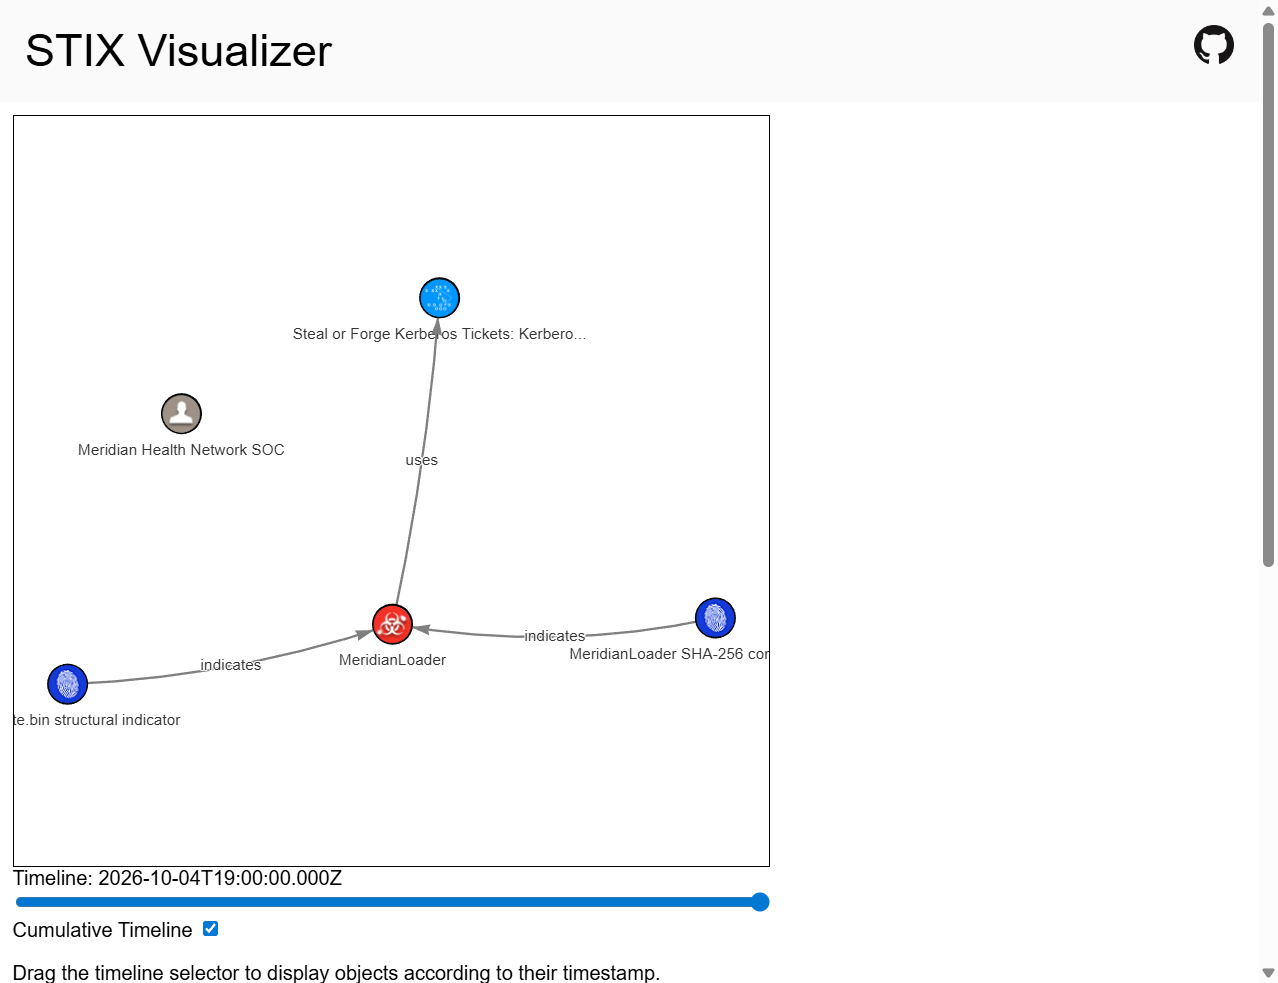
\includegraphics[width=0.92\textwidth,height=0.42\textheight,keepaspectratio]{stix2viz_updated.png}
\end{center}

The graph moved from \textbf{4 nodes / 2 edges} to \textbf{5 nodes / 3 edges}. The new fingerprint-style Indicator node (\texttt{MeridianLoader SHA-256...}) connects into MeridianLoader with an \texttt{indicates} edge; MeridianLoader's hub degree rose from 2 to 3. The timeline includes the new objects' timestamp \texttt{2026-10-04T19:00:00.000Z}.

\labstep{Critical thinking \#3 (challenge graded)}

I chose an \textbf{Indicator} SDO because the new fact is a detection pattern: the SHA-256 of the recovered \texttt{svcupdate.bin} loader. That is not a new malware family, not an ATT\&CK technique, and not a raw \texttt{file} SCO. Indicator is the STIX type that carries a machine-checkable \texttt{pattern} detection tools can load. A lone file SCO would only say the hash was seen; a second Malware object would falsely imply another family; an Attack-Pattern would mislabel a hash as a technique.

I linked it with \texttt{relationship\_type = "indicates"} (Indicator $\rightarrow$ MeridianLoader), not \texttt{related-to} or \texttt{uses}. \texttt{indicates} is the STIX meaning that a pattern match is evidence of that malware. \texttt{uses} would claim the hash employs Kerberoasting; \texttt{related-to} would be a vague link with no detection force. From that SRO a partner may conclude a SHA-256 hit attributes to MeridianLoader---which the Indicator alone does not authorize, because without the relationship the hash is an orphaned sighting with no named malware target. The directed SRO is what makes the hash shared, actionable intel.

\labpart{6. End-to-end workflow}

\begin{center}
\small
\begin{tabular}{@{}c@{ $\rightarrow$ }c@{ $\rightarrow$ }c@{ $\rightarrow$ }c@{ $\rightarrow$ }c@{}}
Author bundle & Validate & stix2viz & medallion & taxii2-client \\
\end{tabular}
\end{center}

The client retrieval matching the authored IDs closes the loop: what was published is what a partner would receive.

\end{document}
